\documentclass{sig-alternate}
%\documentclass{acm_proc_article-sp}

%\makeatletter
%\newif\if@restonecol

%\let\algorithm\relax
%\let\endalgorithm\relax
%\usepackage[tight,footnotesize]{subfigure}

\usepackage {paralist}
\usepackage{comment}
\usepackage{cite}
%\usepackage[cmex10]{amsmath}
\usepackage{subfigure}
\usepackage{url}
%\usepackage{array}
%\usepackage{amsmath}
\usepackage{graphicx}
%\usepackage{amssymb}
\usepackage{cite}
\usepackage{url}
%\makeatother
%\makeatletter
%\providecommand{\tabularnewline}{\\}
\usepackage[ruled]{algorithm2e}


\newtheorem{clm}{Claim}

\begin{document}

\title{STM Concurrency Control for Embedded Real-Time Software with Tighter Time Bounds}


%\author{Mohammed Elshambakey
%\affil{ECE Dept., Virginia Tech, Blacksburg, VA 24060, USA}
%Binoy Ravindran
%\affil{ECE Dept., Virginia Tech, Blacksburg, VA 24060, USA}
%}

\begin{comment}
\author{\IEEEauthorblockN{Mohammed Elshambakey}
\IEEEauthorblockA{ECE Dept, Virginia Tech\\
Blacksburg, VA 24061, USA\\
Email: shambake@vt.edu}
\and
\IEEEauthorblockN{Binoy Ravindran}
\IEEEauthorblockA{ECE Dept, Virginia Tech\\
Blacksburg, VA 24061, USA\\
Email: binoy@vt.edu}
}
\end{comment}


\maketitle

\begin{abstract}
We consider software transactional memory (STM) concurrency control for multicore real-time software, and present a novel contention manager (CM) for resolving transactional conflicts, called length-based CM (or LCM). We upper bound transactional retries and response times under LCM, when used with G-EDF and  G-RMA schedulers. We identify the conditions under which LCM outperforms previous real-time STM CMs and lock-free synchronization. Our implementation and experimental studies reveal that G-EDF/LCM and G-RMA/LCM have shorter or comparable retry costs and response times than other synchronization techniques.
\end{abstract}

%\maketitle

\section{Introduction}
\label{sec:intro}

Lock-based concurrency control suffers from programmability, scalability, and composability challenges~\cite{Herlihy:2006:AMP:1146381.1146382}. These challenges are exacerbated in emerging multicore architectures, on which improved software performance must be achieved by exposing greater concurrency.  Transactional memory (TM) is an alternative synchronization model for shared memory objects that promises to alleviate these difficulties.  With TM, programmers organize code that read/write shared objects as transactions, which appear to execute atomically. Two transactions conflict if they access the same object and one access is a write. When that happens, a contention manager (or CM)
%~\cite{Guerraoui:2005:TTT:1073814.1073863} 
resolves the conflict by aborting one and allowing the other to commit, yielding (the illusion of) atomicity. 
%Aborted transactions are re-started.
%often immediately.  
In addition to a simple programming model, TM provides performance comparable to highly concurrent fine-grained locking and lock-free approaches,  
%~\cite{Saha:2006:MHP:1122971.1123001}, 
and is composable. 
%~\cite{Harris:2005:CMT:1065944.1065952}. 
TM has been proposed in hardware, called HTM,  
%(e.g.,~\cite{austenmc:tcc:dissertation:2009}), 
and in software, called STM,  
%(e.g.,~\cite{sha95}),  
with the usual tradeoffs: HTM has lesser overhead, but needs transactional support in hardware; STM is available on any hardware. See~\cite{tm-book10} for an excellent overview on TM.


Given STM's programmability, scalability, and composability advantages, we consider it for concurrency control in multicore real-time software. Doing so requires bounding transactional  retries, as real-time threads, which subsume transactions, must satisfy time constraints.  Retry bounds in STM are dependent on the CM policy at hand. Thus, real-time CM is logical.

Past research on real-time CM have proposed resolving transactional contention using dynamic and fixed priorities of parent threads, resulting in Earliest-Deadline-First-based CM (ECM) and Rate Monotonic Assignment-based CM~(RCM), respectively~\cite{fahmy2009bounding,fahmy2009response,stmconcurrencycontrol:emsoft11}.
These works show that, ECM and RCM, when used with the Global EDF (G-EDF) and Global RMA  (G-RMA) multicore schedulers, respectively, achieve higher schedulability than lock-free synchronization techniques only under some ranges for the maximum atomic section length. This raises a fundamental question: is it possible to increase the atomic section length by an alternative CM design, so that STM's schedulability advantage has a larger coverage? 

We answer this question by designing a novel CM that can be used with both dynamic and fixed priority (global) multicore real-time schedulers: length-based CM or LCM (Section~\ref{sec 9.1}). LCM resolves conflicts based on the priority of conflicting jobs, besides the length of the interfering atomic section, and the length of the interfered atomic section.  We establish LCM's retry and response time upper bounds, when used with G-EDF (Section~\ref{response g-edf/lcm}) and with G-RMA (Section~\ref{rma}) schedulers. We identify the conditions under which G-EDF/LCM outperforms ECM (Section~\ref{performance g-edf-lcm}) and lock-free synchronization (Section~\ref{gedf-lcm-lock-free}), and G-RMA/LCM outperforms RCM (Section~\ref{rma eval}).

We implement LCM and competitor CM techniques in the Rochester STM framework~\cite{marathe2006lowering} and conduct experimental studies (Section~\ref{exp_eval}). Our study reveals that G-EDF/LCM and G-RMA/LCM have shorter or comparable retry costs and response times than competitors. 

Thus, the paper's contribution is LCM with superior timeliness properties. This result thus allows programmers to reap STM's significant programmability and composability benefits for a broader range of multicore embedded real-time software than what was previously possible.


\section{Related Work}
\label{sec:past}

Transactional-like concurrency control without using locks, for real-time systems, has been previously studied in the context of non-blocking data structures (e.g.,~\cite{anderson95realtime}). Despite their numerous advantages over locks 
(e.g., deadlock-freedom), 
their programmability has remained a challenge. 
Past studies show that they are best suited for simple data structures where their retry cost is competitive to the cost of lock-based synchronization~\cite{bc+08}.  In contrast, STM is semantically simpler~\cite{Herlihy:2006:AMP:1146381.1146382}, and is often the only viable lock-free solution for complex data structures (e.g., red/black tree)~\cite{key-1} and nested critical sections~\cite{Saha:2006:MHP:1122971.1123001}.

STM concurrency control for real-time systems has been previously studied in~\cite{manson2006preemptible,fahmy2009bounding,sarni2009real,schoeberl2010rttm,key-1,barrosmanaging,stmconcurrencycontrol:emsoft11}.


\cite{manson2006preemptible} proposes a restricted version of STM for uniprocessors. Uniprocessors do not need contention management.

\cite{fahmy2009bounding} bounds response times in distributed  systems with STM synchronization. They consider Pfair scheduling, limit to small atomic regions with fixed size, and limit transaction execution to span at most two quanta. In contrast, we allow transaction lengths with  arbitrary duration. 

\cite{sarni2009real} presents real-time scheduling of transactions and serializes transactions based on deadlines. However, the work does not bound retries and response times. In contrast, we establish such bounds.


\cite{schoeberl2010rttm} proposes real-time HTM. The work does not describe how transactional conflicts are resolved. Besides, the retry bound assumes that the worst case conflict between atomic sections of different tasks occurs when the sections are released at the same time. However, we show that this is not the worst case. We develop retry and response time upper bounds based on much worse conditions.


\cite{key-1} upper bounds retries and response times for  ECM with G-EDF, and identify the tradeoffs with locking and lock-free protocols. Similar to~\cite{schoeberl2010rttm},~\cite{key-1} also assumes that the worst case conflict between atomic sections occurs when the sections are released simultaneously. 

The ideas in~\cite{key-1} are extended in~\cite{barrosmanaging}, which presents three real-time CM designs. But no retry bounds or schedulability analysis techniques are presented for those CMs. 

\cite{stmconcurrencycontrol:emsoft11} 
presents the ECM and RCM contention managers, and upper bounds transactional retries and response times under them. The work also identifies the conditions under which ECM and RCM are superior to lock-free synchronization. In particular, they show that, STM's superiority holds only under some ranges for the maximum atomic section length. Our work builds upon this result.

\section{Preliminaries}
\label{sec:model}

We consider a multiprocessor system with $m$ identical processors and $n$ sporadic tasks $\tau_1, \tau_2,\ldots, \tau_n$. The $k^{th}$ instance (or job) of a task $\tau_i$ is denoted $\tau_i^k$. Each task $\tau_i$ is specified by its worst case execution time (WCET) $c_i$, its minimum period $T_i$ between any two consecutive instances, and its relative deadline $D_i$, where $D_i=T_i$. Job $\tau_i^j$ is released at time $r_i^j$ and must finish no later than its absolute deadline $d_i^j=r_i^j+D_i$. Under a fixed priority scheduler such as G-RMA, $p_i$ determines $\tau_i$'s (fixed) priority and it is constant for all instances of $\tau_i$. Under a dynamic priority scheduler such as G-EDF, a job $\tau_i^j$'s priority, $p_i^j$, differs from one instance to another. 
A task $\tau_j$ may interfere with task $\tau_i$ for a number of times during an interval $L$, and this number is denoted as $G_{ij}(L)$. 


\textit{Shared objects.}
 A task may need to read/write shared, in-memory data objects while it is executing any of its atomic sections, which are synchronized using STM. 
The set of atomic sections of task $\tau_i$ is denoted $s_i$. $s_i^k$ is the $k^{th}$ atomic section of $\tau_i$. 
Each object, $\theta$, can be accessed by multiple tasks. The set of distinct objects accessed by $\tau_i$ is $\theta_i$ without repeating objects.
The set of atomic sections used by $\tau_i$ to access $\theta$ is $s_i(\theta)$, and the sum of the lengths of those atomic sections is $len(s_i(\theta))$. $s_i^k(\theta)$ is the $k^{th}$ atomic section of $\tau_i$ that accesses $\theta$. $s_i^k(\theta)$  executes for a duration $len(s_i^k(\theta))$.
% which is the whole length of the atomic section (and not just the part that accesses $\theta$). 
%Thus, for two objects $\theta_1$ and $\theta_2$ that are accessed within the same atomic section of $T_i$, $len(s_i^k(\theta1))=len(s_i^k(\theta2))$. 
%If $\theta$ is shared by multiple tasks, then $s(\theta)$ is the set of atomic sections of all tasks accessing $\theta$, and 
The set of tasks sharing $\theta$ with $\tau_i$ is denoted $\gamma_i(\theta)$. 

Atomic sections are non-nested (supporting nested STM is future work). Each section is assumed to access only one object; this allows us to be consistent with the assumptions in~\cite{stmconcurrencycontrol:emsoft11}, enabling a comparison with retry-loop lock-free synchronization~\cite{key-5}, which is an important goal of this paper.
The maximum-length atomic section in $\tau_i$ that accesses $\theta$ is denoted $s_{i_{max}} (\theta)$, while the maximum one among all tasks is $s_{max} (\theta)$, and the maximum one among tasks with priorities lower than that of $\tau_i$ is $s_{max}^i (\theta)$.

\textit{STM retry cost.} If two or more atomic sections conflict, the CM will commit one section and abort and retry the others, increasing the time to execute the aborted sections. The increased time that an atomic section $s_i^p (\theta)$ will take to execute due to a conflict with another section $s_j^k (\theta)$, is denoted $W_{i}^{p}(s_{j}^{k}(\theta))$. If an atomic section, $s_i^p$, is already executing, and another atomic section $s_j^k$ tries to access a shared object with $s_i^p$, then $s_j^k$ is said to ``interfere" or ``conflict" with $s_i^p$. The job $s_j^k$ is the ``interfering job", and the job $s_i^p$ is the ``interfered job."  
The total time that a task $\tau_i$'s atomic sections have to retry over $T_i$ is denoted $RC(T_i)$.
The additional amount of time that a task $\tau_j$ causes to response time of $\tau_i$ 
when interfering with $\tau_i$ during $L$, without considering retries due to atomic sections, is denoted $W_{ij}(L)$.

\section{Length-based CM}

LCM resolves conflicts based on the priority of conflicting jobs, besides the length of the interfering atomic section, and the length of the interfered atomic section. This is in contrast to ECM and RCM~\cite{stmconcurrencycontrol:emsoft11}, where conflicts are resolved using the priority of the conflicting jobs. This strategy allows lower priority jobs, under LCM, to retry for lesser time than that under ECM and RCM, but higher priority jobs, sometimes, wait for lower priority ones with bounded priority-inversion.

\subsection{\label{sec 9.1} Design and Rationale}

%Begin algorithm here
\begin{algorithm}
\footnotesize{
\LinesNumbered
\KwData{$s_i^k(\theta)\rightarrow$ interfered atomic section.\\$s_j^l(\theta)\rightarrow$ interfering atomic section.\\$\psi\rightarrow$ predefined threshold $\in [0,1]$.\\$\delta_i^k(\theta)\rightarrow$ remaining execution length of $s_i^k(\theta)$}
\KwResult{which atomic section of $s_i^k(\theta)$ or $s_j^l(\theta)$ aborts}
\eIf{$p_i^k > p_j^l$}
	{$s_j^l(\theta)$ aborts\label{step_sicommits}\;}
	{$c_{ij}^{kl}=len(s_j^l(\theta))/len(s_i^k(\theta))$\label{step_cijkl}\;
	$\alpha_{ij}^{kl}=ln(\psi)/(ln(\psi)-c_{ij}^{kl})$\label{step_alphaijkl}\;
	$\alpha=\left(len(s_i^k(\theta))-\delta_i^k(\theta)\right)/len(s_i^k(\theta))$\;
	\eIf{$\alpha \le \alpha_{ij}^{kl}$}
	{$s_i^k(\theta)$ aborts\label{step_siaborts}\;}
	{$s_j^l(\theta)$ aborts\label{step_sjaborts}\;}
	}
	}
\caption{LCM}
\label{alg_lcm}
\end{algorithm}
%End algorithm here

For both ECM and RCM, $s_{i}^{k}(\theta)$ can be totally repeated if $s_{j}^{l}(\theta)$ --- which belongs to a higher priority job $\tau_{j}^b$ than $\tau_{i}^a$ --- conflicts with $s_{i}^{k}(\theta)$
at the end of its execution, while $s_{i}^{k}(\theta)$ is just about
to commit. Thus, LCM, shown in Algorithm~\ref{alg_lcm}, uses the remaining length of $s_{i}^{k}(\theta)$ when it is interfered,
as well as $len(s_{j}^{l}(\theta))$, to decide which transaction must be aborted. If $p_i^k$ was greater than $p_j^l$, then $s_i^k(\theta)$ would be the one that commits, because it belongs to a higher priority job, and it started before $s_j^l(\theta)$ (step~\ref{step_sicommits}). Otherwise, $c_{ij}^{kl}$ is calculated (step~\ref{step_cijkl}) to determine whether it is worth aborting $s_i^k(\theta)$ in favor of $s_j^l(\theta)$, because $len(s_j^l(\theta))$ is relatively small compared to the remaining execution length of $s_i^k(\theta)$  (explained further).

We assume that:
\begin{equation}
c_{ij}^{kl}=len(s_{j}^{l}(\theta))/len(s_{i}^{k}(\theta))
\label{cm_eq}\end{equation}
where $c_{ij}^{kl}\in]0,\infty[$, to cover all possible lengths of $s_{j}^{l}(\theta)$.
Our idea is to reduce the opportunity for the abort of $s_{i}^{k}(\theta)$ if it is close to committing when interfered and $len(s_{j}^{l}(\theta))$ is large. This abort opportunity is increasingly reduced as $s_{i}^{k}(\theta)$ gets closer to the end of its execution, or $len(s_{j}^{l}(\theta))$ gets larger. 

On the other hand, as $s_{i}^{k}(\theta)$ is interfered early,
or $len(s_{j}^{l}(\theta))$ is small compared to $s_{i}^{k}(\theta)$'s remaining length, the abort opportunity 
is increased even if $s_i^k (\theta)$ is close to the end of its execution. To decide whether $s_{i}^{k}(\theta)$ must be aborted or not, we use a threshold value $\psi\in[0,1]$ that determines $\alpha_{ij}^{kl}$ (step~\ref{step_alphaijkl}), where $\alpha_{ij}^{kl}$ is the maximum percentage of $len(s_i^k(\theta))$ below which $s_j^l(\theta)$ is allowed to abort $s_i^k(\theta)$. Thus, if the already executed part of $s_i^k(\theta)$ --- when $s_j^l(\theta)$ interferes with $s_i^k(\theta)$ --- does not exceed $\alpha_{ij}^{kl}len(s_i^k(\theta))$, then $s_i^k(\theta)$ is aborted (step~\ref{step_siaborts}). Otherwise, $s_j^l(\theta)$ is aborted (step~\ref{step_sjaborts}).

%
\begin{figure}[htbp]
\centering
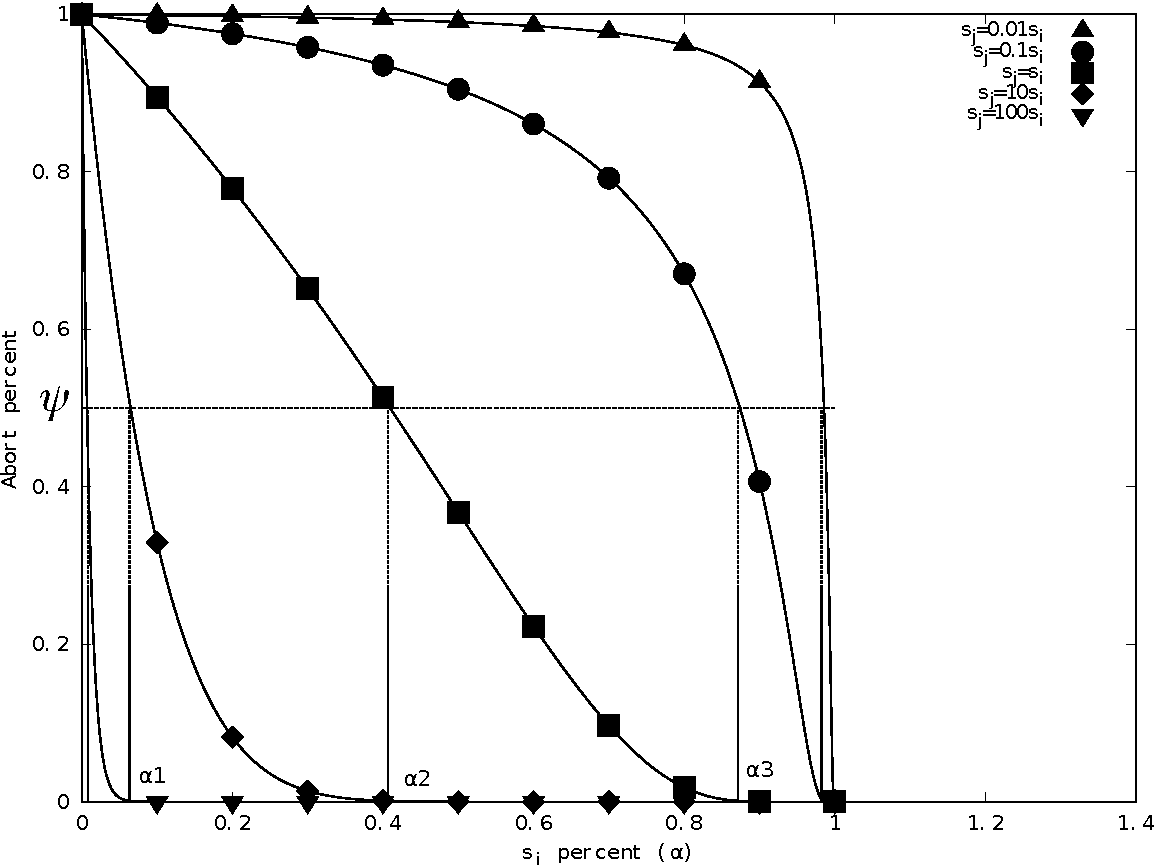
\includegraphics[scale=0.4]{figures/figure16}
\caption{\label{fig16}Interference of $s_{i}^{k}(\theta)$ by various lengths of 
$s_{j}^{l}(\theta)$}
\end{figure}

The behavior of LCM is illustrated in Figure~\ref{fig16}. In this figure, the horizontal axis corresponds to different values of $\alpha$ ranging from $0$ to $1$, and the vertical axis corresponds to different values of abort opportunities, $f(c_{ij}^{kl},\alpha)$, ranging from $0$ to $1$ and calculated by~(\ref{eq49}):
\begin{equation}
f(c_{ij}^{kl},\alpha)=e^{\frac{-c_{ij}^{kl}\alpha}{1-\alpha}}
\label{eq49}\end{equation}
where $c_{ij}^{kl}$ is calculated by~(\ref{cm_eq}).

Figure~\ref{fig16} shows one atomic section $s_i^k(\theta)$ (whose $\alpha$ changes along the horizontal axis) interfered by five different lengths of $s_j^l(\theta)$.
For a predefined value of $f(c_{ij}^{kl},\alpha)$ (denoted as $\psi$ in Algorithm~\ref{alg_lcm}), there corresponds a specific value of $\alpha$ (which is $\alpha_{ij}^{kl}$ in Algorithm~\ref{alg_lcm}) for each curve. For example, when $len(s_j^l(\theta))=0.1 \times len(s_i^k(\theta))$, $s_j^l(\theta)$ aborts $s_i^k(\theta)$ if the latter has not executed more than $\alpha3$ percentage (shown in Figure~\ref{fig16}) of its execution length. As $len(s_{j}^{l}(\theta))$ decreases, the corresponding $\alpha_{ij}^{kl}$ increases (as shown in Figure~\ref{fig16}, $\alpha3>\alpha2>\alpha1$).

Equation (\ref{eq49}) achieves the desired requirement that the abort opportunity is reduced as $s_{i}^{k}(\theta)$ gets
closer to the end of its execution (as $\alpha\rightarrow1,\, f(c_{ij}^{kl},1)\rightarrow0$),
or as the length of the conflicting transaction increases (as $c_{ij}^{kl}\rightarrow\infty,\, f(\infty,\alpha)\rightarrow0$).
Meanwhile, this abort opportunity is increased as $s_{i}^{k}(\theta)$
is interfered closer to its release (as $\alpha\rightarrow0,\, f(c_{ij}^{kl},0)\rightarrow1$),
or as the length of the conflicting transaction decreases (as $c_{ij}^{kl}\rightarrow0,\, f(0,\alpha)\rightarrow1$).

LCM is not a centralized CM, which means that, upon a conflict, each transactions has to decide whether it must commit or abort. 

\begin{clm}
\label{LCM_higher_rc}
Let $s_{j}^{l}(\theta)$ interfere once with $s_{i}^{k}(\theta)$ at $\alpha_{ij}^{kl}$. Then, the maximum contribution of $s_{j}^{l}(\theta)$ to 
$s_{i}^{k}(\theta)$'s 
retry cost is:
\begin{equation}
W_i^k(s_j^l(\theta))\le \alpha_{ij}^{kl}len\Big(s_{i}^{k}(\theta)\Big)+len\Big(s_{j}^{l}(\theta)\Big)\label{eq47}\end{equation}
\end{clm}
(Proofs of all claims are provided in the Supplementary Material section at the end of the paper.)


\begin{clm}
\label{LCM_lower_rc}
An atomic section of a higher priority job, $\tau_{j}^b$, may have to abort and retry due to a lower priority job, $\tau_{i}^a$, if $s_{j}^{l}(\theta)$ interferes
with $s_{i}^{k}(\theta)$ after the $\alpha_{ij}^{kl}$ percentage. $\tau_{j}$'s retry time, due to $s_{i}^{k}(\theta)$ and $s_{j}^{l}(\theta)$,
is upper bounded by:
 \begin{equation}
W_j^l(s_i^k(\theta))\le \Big(1-\alpha_{ij}^{kl}\Big)len\Big(s_{i}^{k}(\theta)\Big)\label{eq48}\end{equation}
\end{clm}

\begin{clm}
\label{priority_inversion}
A higher priority job, $\tau_i^z$, suffers from priority inversion for at most the number of atomic sections in $\tau_i^z$.
\end{clm}


\begin{clm}
\label{max_pri_inv}
The maximum delay suffered by $s_j^l(\theta)$ due to priority inversion is caused by the maximum length atomic section accessing object $\theta$, which belongs to a lower priority job than $\tau_j^b$ that owns $s_j^l(\theta)$.
\end{clm}


\subsection{\label{response g-edf/lcm} Response Time of G-EDF/LCM}

%Toward establishing the response time under G-EDF/LCM, we introduce a set of claims.

\begin{clm}\label{GEDF/LCM response time}
$RC(T_i)$ for a task $\tau_i$ under G-EDF/LCM is upper bounded by:
\begin{eqnarray}
RC(T_i) & = & \Bigg(\sum_{\forall \tau_h \in \gamma_i}\sum_{\forall\theta \in \theta_i \wedge \theta_h}\Bigg(\left\lceil\frac{T_{i}}{T_{h}}\right\rceil\sum_{\forall s_{h}^{l}(\theta)}len\Big(s_{h}^{l}(\theta)\Big)\nonumber\\
& + & \alpha_{max}^{hl}len\Big(s_{max}^{h}(\theta)\Big)\Bigg)\Bigg)\nonumber\\
& + & \sum_{\forall s_{i}^{y}(\theta)}\Big(1-\alpha_{max}^{iy}\Big)len\Big(s_{max}^i(\theta)\Big)  
\label{eq78}\end{eqnarray} 
where $\alpha_{max}^{hl}$ is the $\alpha$ value that corresponds to $\psi$ due to the interference of $s_{max}^h(\theta)$ by $s_h^l(\theta)$. $\alpha_{max}^{iy}$ is the $\alpha$ value that corresponds to $\psi$ due to the interference of $s_{max}^i(\theta)$ by $s_i^y(\theta)$.
\end{clm}


Response time of $\tau_{i}$ is calculated by (11) in~\cite{stmconcurrencycontrol:emsoft11}.
\begin{figure}
\begin{centering}
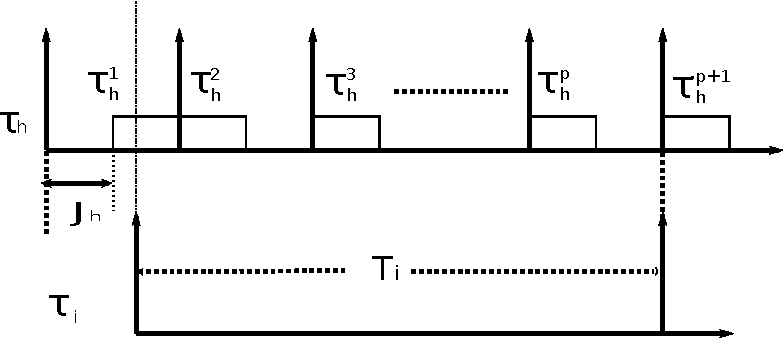
\includegraphics[scale=0.5]{figures/figure18}
\par\end{centering}
\caption{\label{fig17}$\tau_h^p$ has a higher priority than $\tau_i^x$}
\end{figure}

\subsection{Schedulability of G-EDF/LCM and ECM}
\label{performance g-edf-lcm}
We now compare the schedulability of G-EDF/LCM with ECM~\cite{stmconcurrencycontrol:emsoft11} %(FMLP and OMLPprotocols~\cite{key-4,brandenburg2008comparison,key-3}), 
to understand when G-EDF/LCM will perform better. 
Toward this, we compare the total utilization of ECM with that of G-EDF/LCM. For each method, we inflate the $c_i$ of each task $\tau_i$ by adding the retry cost suffered by $\tau_i$. Thus, if method $A$ adds retry cost $RC_A(T_i)$ to $c_i$, and method $B$ adds retry cost $RC_B(T_i)$ to $c_i$, then the schedulability of $A$ and $B$ are compared as:
\begin{eqnarray}
\sum_{\forall \tau_{i}}\frac{c_{i}+RC_A(T_{i})}{T_{i}} & \le & \sum_{\forall \tau_{i}}\frac{c_{i}+RC_B(T_{i})}{T_{i}}\nonumber\\
\sum_{\forall \tau_{i}}\frac{RC_A(T_{i})}{T_{i}} & \le & \sum_{\forall \tau_{i}}\frac{RC_B(T_{i})}{T_{i}}
\label{eqa}\end{eqnarray}
Thus, schedulability is compared by substituting the retry cost added by the synchronization methods in (\ref{eqa}).

\begin{clm}\label{lcm versus ecm}
Let $s_{max}$ be the maximum length atomic section accessing any object $\theta$. Let $\alpha_{max}$ and $\alpha_{min}$ be the maximum and minimum values of $\alpha$ for any two atomic sections $s_i^k(\theta)$ and $s_j^l(\theta)$. Given a threshold $\psi$, schedulability of G-EDF/LCM is equal or better than ECM if for any task $\tau_i$:
\begin{equation}
\frac{1-\alpha_{min}}{1-\alpha_{max}} \le \sum_{\forall \tau_h \in \gamma_i}\left\lceil\frac{T_i}{T_h}\right\rceil
\label{edf-lcm-ecm}\end{equation}
\end{clm}

\subsection{G-EDF/LCM versus Lock-free}
\label{gedf-lcm-lock-free}
We consider the retry-loop lock-free synchronization for G-EDF given in~\cite{key-5}. This lock-free approach is the most relevant to our work. 

\begin{clm}\label{gedf-lcm-lock-free_clm} 
Let $s_{max}$ denote $len(s_{max})$ and $r_{max}$ denote the maximum execution cost of a single iteration of any retry loop of any task in the retry-loop lock-free algorithm in~\cite{key-5}. Now, G-EDF/LCM achieves higher schedulability than the retry-loop lock-free approach if the upper bound on $s_{max}/r_{max}$ under G-EDF/LCM ranges between 0.5 and 2 (which is higher than that under  ECM). 
\end{clm}

\subsection{Response Time of G-RMA/LCM}
\label{rma}

\begin{clm}\label{response g-rma/lcm}
Let $\lambda_{2}(j,\theta)=\sum_{\forall s_{j}^{l}(\theta)}len(s_{j}^{l}(\theta))+\alpha_{max}^{jl}len(s_{max}^{j}(\theta))$, where $\alpha_{max}^{jl}$ is the $\alpha$ value corresponding to $\psi$ due to the interference of $s_{max}^j(\theta)$ by $s_j^l(\theta)$. The retry cost of any task $\tau_i$ under G-RMA/LCM during $T_i$ 
is given by:
\begin{eqnarray}
RC\left(T_i\right) & = &
  \sum_{\forall \tau_{j}^{*}}\left(\sum_{\theta\in(\theta_{i}\wedge\theta_{j})}\left(\left(\left\lceil\frac{T_i}{T_{j}}\right\rceil +1\right)\lambda_{2}(j,\theta)\right)\right)\nonumber\\
& + & \sum_{\forall s_{i}^{y}(\theta)}\Big(1-\alpha_{max}^{iy}\Big)len\Big(s_{max}^i(\theta)\Big)
\label{eq60}
\end{eqnarray}
where $\tau_{j}^{*}=\{\tau_{j}|(\tau_{j}\in\gamma_{i})\wedge(p_{j}>p_{i})\}$.
\end{clm}

The response time is calculated by (17) in~\cite{stmconcurrencycontrol:emsoft11} with replacing $RC(R_i^{up})$ with $RC(T_i)$.
%BR: You should say "..with $RC(T_i)$ replacing $RC(R_i^{up})$."

\subsection{Schedulability of G-RMA/LCM and RCM}
\label{rma eval}

\begin{clm}\label{rma_eval_clm}
Under the same assumptions of Claims~\ref{lcm versus ecm} and~\ref{response g-rma/lcm}, G-RMA/LCM's schedulability is equal or better than RCM if:
\begin{equation}
\frac{1-\alpha_{min}}{1-\alpha_{max}}\le \sum_{\forall \tau_j^*}\left( \left\lceil\frac{T_i}{T_j}\right\rceil +1 \right)
\label{eq70}\end{equation}
\end{clm}

\section{Experimental Evaluation}\label{exp_eval}

Having established LCM's retry and response time upper bounds, and the conditions under which it outperforms ECM, RCM, and lock-free synchronization, we now would like to understand how LCM's retry and response times in practice (i.e., on average) compare with that of competitor methods. Since this can only be understood experimentally, we implement LCM and the competitor methods and conduct experimental studies. 

\subsection{Experimental Setup}
We used the ChronOS real-time Linux kernel~\cite{dellinger2011chronos}
and the RSTM library~\cite{marathe2006lowering}. We modified RSTM to include implementations of ECM, RCM, G-EDF/LCM, and G-RMA/LCM contention managers, and modified ChronOS to include implementations of G-EDF and G-RMA schedulers. 

For the retry-loop lock-free implementation,
we used a loop that reads an object and attempts to write to the object using a compare-and-swap (CAS) instruction. The task retries until the CAS succeeds. 
%We call this lock-free operation, CAS-loop operation.

We use an 8 core, 2GHz AMD Opteron platform. The average time
taken for one write operation by RSTM on any
core is 0.0129653375$\mu s$, and the average time taken
by one CAS-loop operation on any core is 0.0292546250 $\mu s$.

We used the periodic task set shown in Table~\ref{tab:Task-set-1}. Each task runs in its own thread and has an atomic section. Atomic section properties are probabilistically controlled (for experimental evaluation) using three parameters: the maximum and minimum lengths of any atomic section within the task, and the total length of atomic sections within any task. All task atomic sections access the same object, and do write operations on the object (thus, contention is the highest).


To compare STM with the retry-loop lock-free method, the same length of each atomic section within any task is implemented using the CAS-loop operation. 
This allows us to compare the effect of contention resolution between the  STM and lock-free methods, ignoring the overhead of their implementations.

\begin{table}
\caption{\label{tab:Task-set-1}Task sets. (a) \label{tab:Task-sets-(a)} Task set 1: 5-task set; 
\label{tab:Task-sets-(b)} (b) Task set 2: 10-task set; \label{tab:Task-sets-(c)} (c) Task set 3: 12-task set}
\centering{}\begin{tabular}{|c|c|c|}
\multicolumn{3}{c}{(a)}\tabularnewline
\cline{2-3} 
\multicolumn{1}{c|}{} & $T_{i}(\mu s)$ & $c_{i}(\mu s)$\tabularnewline
\hline 
$\tau_{1}$ & 500000 & 150000\tabularnewline
\hline 
$\tau_{2}$ & 1000000 & 227000\tabularnewline
\hline 
$\tau_{3}$ & 1500000 & 410000\tabularnewline
\hline 
$\tau_{4}$ & 3000000 & 299000\tabularnewline
\hline 
$\tau_{5}$ & 5000000 & 500000\tabularnewline
\hline
\end{tabular} \begin{tabular}{|c|c|c|}
\multicolumn{3}{c}{(b)}\tabularnewline
\cline{2-3} 
\multicolumn{1}{c|}{} & $T_{i}(\mu s)$ & $c_{i}(\mu s)$\tabularnewline
\hline 
$\tau_{1}$ & 400000 & 75241\tabularnewline
\hline 
$\tau_{2}$ & 750000 & 69762\tabularnewline
\hline 
$\tau_{3}$ & 1200000 & 267122\tabularnewline
\hline 
$\tau_{4}$ & 1500000 & 69863\tabularnewline
\hline 
$\tau_{5}$ & 2400000 & 152014\tabularnewline
\hline 
$\tau_{6}$ & 4000000 & 286301\tabularnewline
\hline 
$\tau_{7}$ & 7500000 & 493150\tabularnewline
\hline 
$\tau_{8}$ & 10000000 & 794520\tabularnewline
\hline 
$\tau_{9}$ & 15000000 & 1212328\tabularnewline
\hline 
$\tau_{10}$ & 20000000 & 1775342\tabularnewline
\hline
\end{tabular} \begin{tabular}{|c|c|c|}
\multicolumn{3}{c}{(c)}\tabularnewline
\cline{2-3} 
\multicolumn{1}{c|}{} & $T_{i}(\mu s)$ & $c_{i}(\mu s)$\tabularnewline
\hline 
$\tau_{1}$ & 400000 & 58195\tabularnewline
\hline 
$\tau_{2}$ & 750000 & 53963\tabularnewline
\hline 
$\tau_{3}$ & 1000000 & 206330\tabularnewline
\hline 
$\tau_{4}$ & 1200000 & 53968\tabularnewline
\hline 
$\tau_{5}$ & 1500000 & 117449\tabularnewline
\hline 
$\tau_{6}$ & 2400000 & 221143\tabularnewline
\hline 
$\tau_{7}$ & 3000000 & 290428\tabularnewline
\hline 
$\tau_{8}$ & 4000000 & 83420\tabularnewline
\hline 
$\tau_{9}$ & 7500000 & 380917\tabularnewline
\hline 
$\tau_{10}$ & 10000000 & 613700\tabularnewline
\hline 
$\tau_{11}$ & 15000000 & 936422\tabularnewline
\hline 
$\tau_{12}$ & 20000000 & 1371302\tabularnewline
\hline
\end{tabular}
\end{table}

\subsection{Results}

Figure \ref{fig:RC_results} shows the retry cost (RC) 
for each task in the three task sets in Table \ref{tab:Task-set-1}, where each task's atomic section length is equal to half of the task length.
%%BR: What are the confidence intervals of each data point? Describe that here: "Each data point in the figure has a confidence interval of ...."
We observe that G-EDF/LCM and G-RMA/LCM achieve shorter
or comparable retry cost than ECM and RCM. Since all tasks are initially
released at the same time, and due to the specific nature of task properties, tasks with lower IDs somehow have higher priorities under the G-EDF scheduler. Note that tasks with lower IDs have higher priorities under G-RMA, since tasks are ordered in non-decreasing order of their periods. 

Thus, we observe that G-EDF/LCM and G-RMA/LCM achieve comparable retry costs
to ECM and RCM for some tasks with lower IDs. But when task ID increases,
LCM --- for both schedulers --- achieves much shorter retry costs 
than ECM and RCM. 
This is because, higher priority tasks in LCM suffers blocking
by lower priority tasks, which is not the case for ECM and RCM. However, as task priority decreases, LCM, by definition, prevents higher priority
tasks from aborting lower priority ones if a higher priority task
interferes with a lower priority one after a specified threshold. In contrast, under ECM and RCM, lower priority tasks abort in favor of higher priority ones. G-EDF/LCM and G-RMA/LCM also achieve comparable or shorter retry costs than the retry-loop lock-free algorithm.

\begin{figure}[htbp]
\centering
\subfigure[Task set 1]{
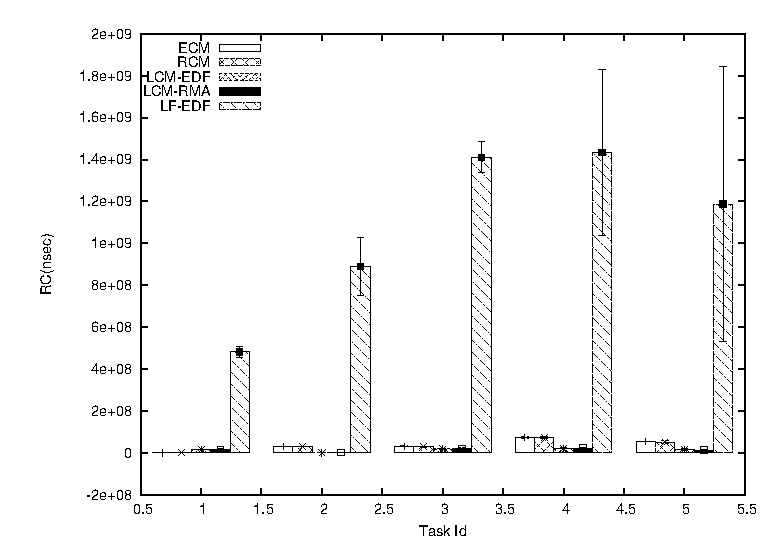
\includegraphics[scale=0.7]
{figures/Abr_dur_5t_nl_g_30_0.5_0.5_0.5_1.eps}
\label{fig-RC-set1}
}
\subfigure[Task set 2]{
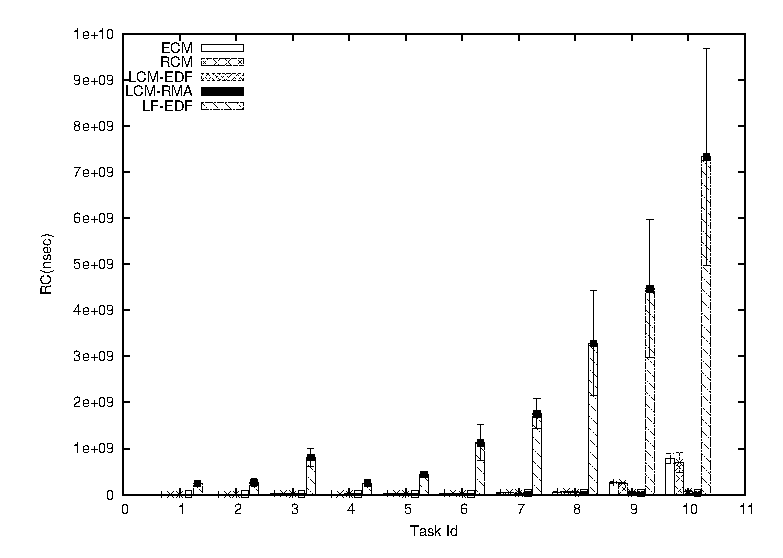
\includegraphics[scale=0.7]{figures/Abr_dur_10t_nl_g_30_0.5_0.5_0.5_1.eps}
\label{fig-RC-set2}
}
\subfigure[Task set 3]{
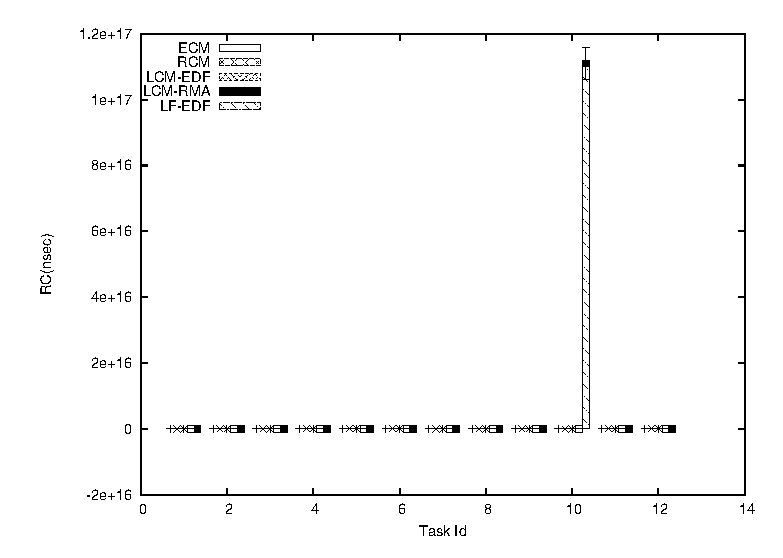
\includegraphics[scale=0.7]{figures/Abr_dur_12t_nl_g_30_0.5_0.5_0.5_1.eps}
\label{fig-RC-set3}
}
\caption{Task retry costs under LCM and competitor synchronization methods}
\label{fig:RC_results}
\end{figure}

Figure \ref{fig:res_results-1} shows the response time of each task in the Table \ref{tab:Task-set-1} task sets. (Again, each task's atomic section length is equal to half of the task length.) 
We observe that G-EDF/LCM and G-RMA/LCM achieve shorter 
response time than the retry-loop lock-free
algorithm, and shorter 
or comparable response time than ECM and RCM.

%%BR: You should indicate that, these results are consistent when other parameters are varied, like the length of the atomic section, # of objects, etc, assuming that you have done those experiments. (Plus, you can also include additional results in the Supplementary Material section.) If you have done them and have seen consistent trends, then you can say here as a (separate paragraph): 
%We repeated the experiments by varying the number of tasks, number and length of atomic sections, and number objects, and observed consistent trends. Full set of results are omitted here due to space constraints; however additional results are included in the Supplementary Material section.

\begin{figure}[htbp]
\subfigure[Task set 1]{
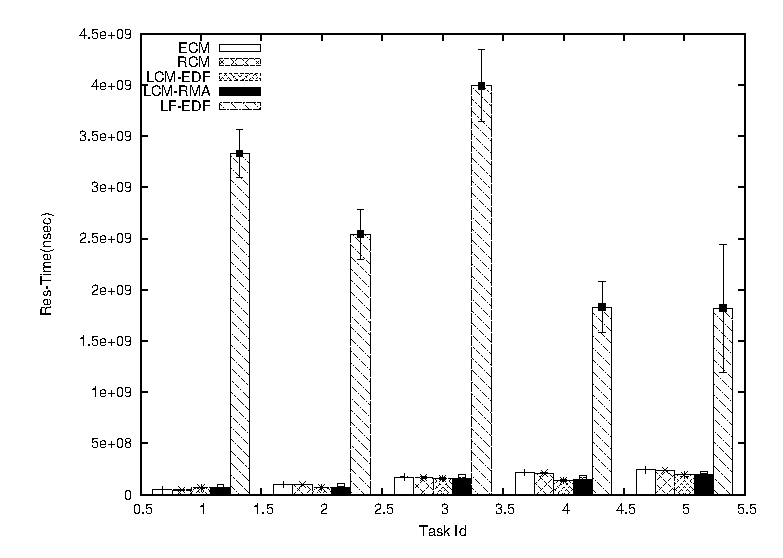
\includegraphics[scale=0.7]{figures/Res_Time_5t_nl_g_30_0.5_0.5_0.5_1.eps}
\label{fig-res-set1-1}
}
\subfigure[Task set 2]{
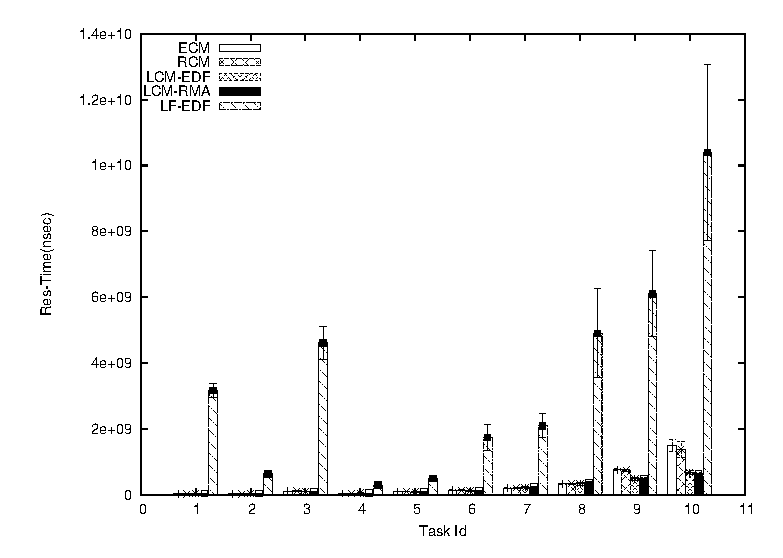
\includegraphics[scale=0.7]{figures/Res_Time_10t_nl_g_30_0.5_0.5_0.5_1.eps}
\label{fig-res-set2-1}
}
\subfigure[Task set 3 ]{
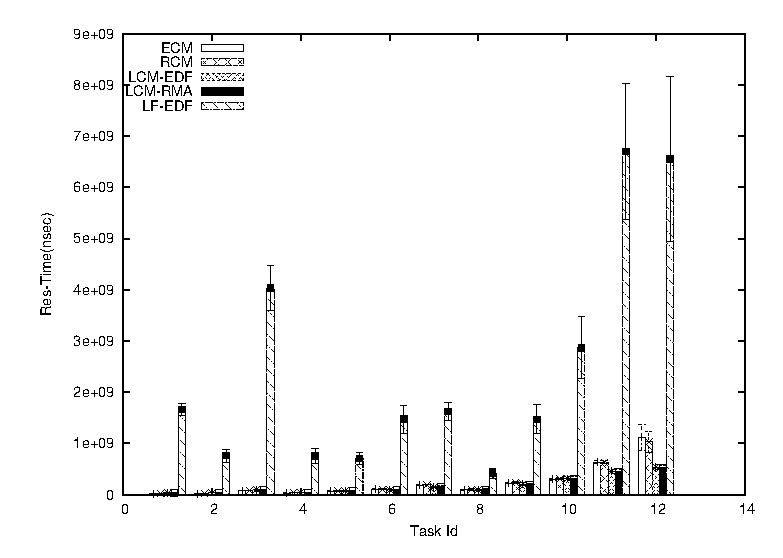
\includegraphics[scale=0.7]{figures/Res_Time_12t_nl_g_30_0.5_0.5_0.5_1.eps}
\label{fig-res-set3-1}
}
\caption{Task response times under LCM and competitor synchronization methods}
\label{fig:res_results-1}
\end{figure}

\section{Conclusions}
\label{sec:conclusions}

In ECM and RCM, a task incurs at most $2s_{max}$ retry cost for each of its atomic section due to conflict
with another task's atomic section. With LCM, this retry cost is reduced to $(1+\alpha_{max})s_{max}$ for each aborted atomic section. In ECM and RCM, tasks do not retry due to lower priority tasks, whereas in LCM, they do so. In G-EDF/LCM, retry due to a lower priority job is encountered only from a task $\tau_{j}$'s last job instance 
during $\tau_{i}$'s period. This is not the case with G-RMA/LCM, because,  each higher priority task can be aborted and retried by any job instance of lower priority tasks. Schedulability of G-EDF/LCM and G-RMA/LCM is better or equal to ECM and RCM, respectively, by proper choices for $\alpha_{min}$ and $\alpha_{max}$. Schedulability of G-EDF/LCM is better than retry-loop lock-free synchronization for G-EDF if the upper bound on $s_{max}/r_{max}$ is between 0.5 and 2, which is higher than that achieved by ECM.

\begin{comment}
Our work has only further scratched the surface of real-time STM. Experimental work reveals the superiority of G-EDF/LCM and G-RMA/LCM to other real time contention managers and retry-loop lock-free concurrency control. Further experiments are needed to answer questions like: what are the typical range of values for the different parameters that affect the retry and blocking costs (and hence response time)? How tight is our derived upper bounds in practice? 
What is the most practically suitable
value for $\psi$, $\alpha_{min}$, and $\alpha_{max}$? Is it more suitable to have different $\psi$s for different atomic section lengths, instead of using a common one? Future work is expected to include multiple objects per atomic section and nested atomic sections.
\end{comment}


%\bibliographystyle{acmsmall}
%\bibliography{global_bibliography}

\bibliographystyle{abbrv}
\bibliography{global_bibliography}

\renewcommand{\thesubsection}{S.\arabic{subsection}}

\section*{Supplementary Material}

This section includes proofs of all Claims.
\subsection{\label{proof_LCM_higher_rc}Proof of Claim~\ref{LCM_higher_rc}}
\begin{proof}
If $s_{j}^{l}(\theta)$ interferes with $s_{i}^{k}(\theta)$
at a $\Upsilon$ percentage, where $\Upsilon<\alpha_{ij}^{kl}$,
then the retry cost of $s_{i}^{k}(\theta)$ is $\Upsilon len(s_{i}^{k}(\theta))+len(s_{j}^{l}(\theta))$, which is lower than that calculated in (\ref{eq47}). Besides, 
if $s_{j}^{l}(\theta)$ interferes with $s_{i}^{k}(\theta)$ after
$\alpha_{ij}^{kl}$ percentage, then $s_{i}^{k}(\theta)$ will not
abort.
\end{proof}
%1
\subsection{\label{proof_LCM_lower_rc} Proof of Claim~\ref{LCM_lower_rc}}
\begin{proof}
It is derived directly from Claim~\ref{LCM_higher_rc}, as $s_j^l(\theta)$ will have to retry for the remaining length of $s_i^k(\theta)$.
\end{proof}
%2
\subsection{\label{proof_priority_inversion} Proof of Claim~\ref{priority_inversion}}
\begin{proof}
Assume three atomic sections, $s_i^k(\theta)$, $s_j^l(\theta)$, and $s_a^b(\theta)$, where $p_j > p_i$ and $s_j^l(\theta)$ interferes with $s_i^k(\theta)$ after $\alpha_{ij}^{kl}$. Then, $s_j^l(\theta)$ will have to abort and retry. At this time, if $s_a^b(\theta)$ interferes with the other two atomic sections, then LCM decides which transaction to commit by comparing the two transactions. So, we have the following cases:
\begin{itemize}
\item $p_a < p_i < p_j$. Now, $s_a^b(\theta)$ will not abort any one because it is still in its beginning and it is of the lowest priority. Thus, $\tau_j$ is not indirectly blocked by $\tau_a$.
\item $p_i<p_a<p_j$. Now, even if $s_a^b(\theta)$ interferes with $s_i^k(\theta)$ before $\alpha_{ia}^{kb}$,  $s_a^b(\theta)$ is allowed to abort $s_i^k(\theta)$. After comparing $s_j^l(\theta)$ and $s_a^b(\theta)$, LCM will select $s_j^l(\theta)$ to commit and abort $s_a^b(\theta)$, because the latter is still at its beginning, and $\tau_j$ is of higher priority. If $s_a^b(\theta)$ is not allowed to abort $s_i^k(\theta)$, the situation is still the same, because $s_j^l(\theta)$ was already retrying until $s_i^k(\theta)$ finishes.
%
\item $p_a>p_j>p_i$. Now, if $s_a^b(\theta)$ is chosen to commit, this will not cause a priority inversion for $\tau_j$ because $\tau_a$ is of higher priority.
\item if $\tau_a$ preempts $\tau_i$, then LCM will compare only between $s_j^l(\theta)$ and $s_a^b(\theta)$. If $p_a<p_j$, then $s_j^l(\theta)$ will commit because of its task's higher priority and $s_a^b(\theta)$ is still at its beginning. Otherwise, $s_j^l(\theta)$ will retry, but this will not be priority inversion, because $\tau_a$ is already of higher priority than $\tau_j$. If $\tau_a$ does not access any object but it preempts $\tau_i$, then LCM will choose $s_j^l(\theta)$ to commit, since only already running transactions are competing together.
\end{itemize}
Thus, by generalizing these cases to any number of conflicting jobs, it can be seen that when an atomic section, $s_j^l(\theta)$, of a higher priority job conflicts with a number of atomic sections belonging to lower priority jobs, $s_j^l(\theta)$ can suffer priority inversion by only one of them. Thus, each higher priority job can suffer priority inversion at most its number of atomic sections. Claim follows.
\end{proof}
%3
%%
\subsection{\label{proof_max_pri_inv} Proof of Claim~\ref{max_pri_inv}}
\begin{proof}
Assume three atomic sections, $s_i^k(\theta)$, $s_j^l(\theta)$, and $s_h^z(\theta)$, where $p_j>p_i$, $p_j>p_h$, and $len(s_i^k(\theta))>len(s_h^z(\theta))$. Now, $\alpha_{ij}^{kl}>\alpha_{hj}^{zl}$ and $c_{ij}^{kl}<c_{hj}^{zl}$. By applying~(\ref{eq48}) to obtain the contribution of $s_i^k(\theta)$ and $s_h^z(\theta)$ to the priority inversion of $s_j^l(\theta)$ and dividing them, we get:
\begin{eqnarray*}
\frac{W_{j}^{l}(s_{i}^{k}(\theta))}{W_{j}^{l}(s_{h}^{z}(\theta))} & = & \frac{\left(1-\alpha_{ij}^{kl}\right)len(s_{i}^{k}(\theta))}{\left(1-\alpha_{hj}^{zl}\right)len(s_{h}^{z}(\theta))}
\end{eqnarray*}
By substitution for $\alpha$s from~(\ref{eq49}):
\begin{eqnarray*}
 & = & \frac{(1-\frac{ln\psi}{ln\psi-c_{ij}^{kl}})len(s_{i}^{k}(\theta))}{(1-\frac{ln\psi}{ln\psi-c_{hj}^{zl}})len(s_{h}^{z}(\theta))}
  =  \frac{(\frac{-c_{ij}^{kl}}{ln\psi-c_{ij}^{kl}})len(s_{i}^{k}(\theta))}{(\frac{-c_{hj}^{zl}}{ln\psi-c_{hj}^{zl}})len(s_{h}^{z}(\theta))}\end{eqnarray*}
$\because ln\psi \le 0$ and $c_{ij}^{kl},c_{hj}^{kl} > 0, \therefore$ by substitution from~(\ref{cm_eq})
\begin{eqnarray*}
 & = & \frac{len(s_{j}^{l}(\theta))/(ln\psi-c_{ij}^{kl})}{len(s_{j}^{l}(\theta))/(ln\psi-c_{hj}^{zl})}
  =  \frac{ln\psi-c_{hj}^{zl}}{ln\psi-c_{ij}^{kl}}>1\end{eqnarray*}
Thus, as the length of the interfered atomic section increases, the effect of priority inversion on the interfering atomic section increases. Claim follows.
\end{proof}
%4
\subsection{\label{proof_GEDF/LCM response time}Proof of Claim~\ref{GEDF/LCM response time}}
\begin{proof}
The maximum number of higher priority instances of $\tau_h$ that can interfere with $\tau_i^x$ is $\left\lceil\frac{T_i}{T_h}\right\rceil$, as shown in Figure~\ref{fig17}, where one instance of $\tau_h$ and $\tau_h^p$ coincides with the absolute deadline of $\tau_i^x$.


By using Claims~\ref{LCM_higher_rc},~\ref{LCM_lower_rc},~\ref{priority_inversion}, and~\ref{max_pri_inv}, and Claim 1 in~\cite{stmconcurrencycontrol:emsoft11} to determine the effect of atomic sections belonging to higher and lower priority instances of interfering tasks to $\tau_i^x$, claim follows.
\end{proof}
%5
\subsection{\label{proof_lcm versus ecm}Proof of Claim~\ref{lcm versus ecm}}
\begin{proof}
Under ECM, $RC(T_{i})$ is upper bounded by:
\begin{equation}
RC(T_{i})\le\sum_{\forall \tau_{h}\in\gamma_{i}}\sum_{\forall \theta\in\ (\theta_{i}\wedge\theta_{h})}\left(\left\lceil\frac{T_{i}}{T_{h}}\right\rceil\sum_{\forall s_{h}^{z}(\theta)}2len(s_{max})\right)\label{eq61}\end{equation}
with the assumption that all lengths of atomic sections of (4) and (8) in~\cite{stmconcurrencycontrol:emsoft11} and~(\ref{eq78}) are replaced by $s_{max}$.
%~\cite{stmconcurrencycontrol:emsoft11}. 
Let $\alpha_{max}^{hl}$ in~(\ref{eq78}) be replaced with $\alpha_{max}$, and $\alpha_{max}^{iy}$ in~(\ref{eq78}) be replaced with $\alpha_{min}$. 
As $\alpha_{max}$, $\alpha_{min}$, and $len(s_{max})$ are all constants, (\ref{eq78}) is upper bounded by:
\begin{eqnarray}
RC(T_i) & \le & \Bigg(\sum_{\forall \tau_h \in \gamma_i}\sum_{\forall\theta \in \theta_i \wedge \theta_h}\Bigg(\left\lceil\frac{T_{i}}{T_{h}}\right\rceil\sum_{\forall s_{h}^{l}(\theta)}\left(1+\alpha_{max}\right)\nonumber\\
& & len\Big(s_{max}\Big)\Bigg)\Bigg)
 +  \sum_{\forall s_{i}^{y}(\theta)}\Big(1-\alpha_{min}\Big)len\Big(s_{max}\Big)\nonumber\\ 
\label{eq101}\end{eqnarray}
%
If $\beta_1^{ih}$ is the total number of times any instance of $\tau_h$ accesses shared objects with $\tau_i$, then $\beta_1^{ih}=\sum_{\forall \theta\in(\theta_{i}\wedge\theta_{h})}\sum_{\forall s_{h}^{z}(\theta)}$. Furthermore, if $\beta_2^i$ is the total number of times any instance of $\tau_i$ accesses shared objects with any other instance,   $\beta_2^i=\sum_{\forall s_{i}^{y}(\theta)}$\textit{, where $\theta$ is shared with another task}. Then, $\beta_{i}=max\{max_{\forall \tau_h \in \gamma_i}\{\beta_1^{ih}\},\beta_2^i\}$ is the maximum number of accesses to all shared objects by any instance of $\tau_{i}$ or $\tau_{h}$. 
Thus, (\ref{eq61}) becomes:
\begin{equation}
RC(T_{i})\le\sum_{\tau_{h}\in\gamma_{i}}2\left\lceil\frac{T_{i}}{T_{h}}\right\rceil\beta_{i}len(s_{max})
\label{eq63}\end{equation}
and (\ref{eq101}) becomes:
\begin{eqnarray}
RC(T_{i}) & \le & \beta_{i}len(s_{max}) \Bigg((1-\alpha_{min})\nonumber\\
& + & \sum_{\forall \tau_h \in \gamma_i}\left\lceil\frac{T_{i}}{T_{h}}\right\rceil(1+\alpha_{max})\Bigg)
\label{eq102}\end{eqnarray}

We can now compare the total utilization of G-EDF/LCM with that of ECM by comparing~(\ref{eq101}) and~(\ref{eq102}) for all $\tau_i$:
\begin{eqnarray}
& & \sum_{\forall \tau_{i}}\frac{(1-\alpha_{min})+\sum_{\forall \tau_{h}\in\gamma_{i}}\left(\left\lceil\frac{T_{i}}{T_{h}}\right\rceil(1+\alpha_{max})\right)}{T_{i}} \nonumber\\
& \le &   \sum_{\forall \tau_{i}}\frac{\sum_{\forall \tau_{h}\in\gamma_{i}}2\left\lceil\frac{T_{i}}{T_{h}}\right\rceil}{T_{i}}\label{eqc}\end{eqnarray}

(\ref{eqc}) is satisfied if for each $\tau_{i}$, the following condition is satisfied:
\begin{equation*}
(1-\alpha_{min})+\sum_{\forall \tau_h \in \gamma_i}\left(\left\lceil\frac{T_{i}}{T_{h}}\right\rceil(1+\alpha_{max})\right)  \le  2\sum_{\forall \tau_h \in \gamma_i}\left\lceil\frac{T_{i}}{T_{h}}\right\rceil
\end{equation*}
\begin{equation*}
\therefore\frac{1-\alpha_{min}}{1-\alpha_{max}}  \le  \sum_{\forall \tau_h \in \gamma_i}\left\lceil\frac{T_{i}}{T_{h}}\right\rceil
\end{equation*}
Claim follows.
\end{proof}
%6

%%
\subsection{\label{proof_gedf-lcm-lock-free_clm}Proof of Claim~\ref{gedf-lcm-lock-free_clm}}
\begin{proof}
From~\cite{key-5}, the retry-loop lock-free algorithm is upper bounded by:
\begin{equation}
RL(T_i)=\sum_{\tau_{h}\in\gamma_{i}}\left(\left\lceil\frac{T_{i}}{T_{h}}\right\rceil +1\right)\beta_{i}r_{max}
\label{eq32}\end{equation}
where $\beta_i$ is as defined in Claim~\ref{lcm versus ecm}.
The retry cost of $\tau_i$ in G-EDF/LCM is upper bounded by (\ref{eq102}). By comparing G-EDF/LCM's total utilization with that of the retry-loop lock-free algorithm, we get:
\begin{eqnarray*}
%& 
& \sum_{\forall \tau_{i}}\frac{\left((1-\alpha_{min})+\sum_{\forall \tau_{h}\in\gamma_{i}}\left(\left\lceil\frac{T_{i}}{T_{h}}\right\rceil(1+\alpha_{max})\right)\right)\beta_{i}s_{max}}{T_{i}}\\
%& 
\le & \sum_{\forall \tau_{i}}\frac{\sum_{\forall \tau_{h}\in\gamma_{i}}\left(\left\lceil\frac{T_{i}}{T_{h}}\right\rceil+1\right)\beta_{i}r_{max}}{T_{i}}\end{eqnarray*}
%
\begin{eqnarray}
\therefore\frac{s_{max}}{r_{max}}\le \frac{\sum_{\forall \tau_{i}}\frac{\sum_{\forall \tau_{h}\in\gamma_{i}}\left(\left\lceil\frac{T_{i}}{T_{h}}\right\rceil+1\right)\beta_{i}}{T_{i}}}{\sum_{\forall \tau_{i}}\frac{\left((1-\alpha_{min})+\sum_{\forall \tau_{h}\in\gamma_{i}}\left(\left\lceil\frac{T_{i}}{T_{h}}\right\rceil(1+\alpha_{max})\right)\right)\beta_{i}}{T_{i}}}
\label{u-gedf-lcm-ecm}\end{eqnarray}

If
\begin{eqnarray}
\frac{s_{max}}{r_{max}}\le \frac{{\sum_{\forall \tau_{h}\in\gamma_{i}}\left(\left\lceil\frac{T_{i}}{T_{h}}\right\rceil+1\right)}}{{(1-\alpha_{min})+\sum_{\forall \tau_{h}\in\gamma_{i}}\left(\left\lceil\frac{T_{i}}{T_{h}}\right\rceil(1+\alpha_{max})\right)}}
\label{t-gedf-lcm-ecm}\end{eqnarray}
for each $\tau_i$, then~(\ref{u-gedf-lcm-ecm}) holds.

Let the number of tasks that have shared objects with $\tau_i$ be $\omega$ (i.e., $\sum_{\tau_h \in \gamma_i}=\omega \ge 1$ since at least one task has a shared object with $\tau_i$; otherwise, there is no conflict between tasks). Let the total number of tasks be $n$, so $1\le \omega \le n-1$, and $\left\lceil\frac{T_i}{T_h}\right\rceil \in [1,\infty[$. To find the minimum and maximum values 
for the upper bound on $s_{max}/r_{max}$, we consider the following cases:
\begin{itemize}
\item $\alpha_{min} \rightarrow 0, \alpha_{max} \rightarrow 0$
\end{itemize}
$\therefore$~(\ref{t-gedf-lcm-ecm}) will be:
\begin{eqnarray}
\frac{s_{max}}{r_{max}} & \le & \frac{{\sum_{\forall \tau_{h}\in\gamma_{i}}\left(\left\lceil\frac{T_{i}}{T_{h}}\right\rceil+1\right)}}{{1+\sum_{\forall \tau_{h}\in\gamma_{i}}\left\lceil\frac{T_{i}}{T_{h}}\right\rceil}}
 =  1+\frac{\omega-1}{1+\sum_{\forall \tau_h \in \gamma_i}\left\lceil\frac{T_i}{T_h}\right\rceil}\nonumber\\
\label{s-r-1}\end{eqnarray}
By substituting the edge values for $\omega$ and $\left\lceil\frac{T_i}{T_h}\right\rceil$ in~(\ref{s-r-1}), we derive that the upper bound on $s_{max}/r_{max}$ lies between 1 and 2.

\begin{itemize}
\item $\alpha_{min} \rightarrow 0, \alpha_{max} \rightarrow 1$
\end{itemize}
(\ref{t-gedf-lcm-ecm}) becomes
\begin{eqnarray}
\frac{s_{max}}{r_{max}} & \le & 0.5+ \frac{\omega - 0.5}{1+\sum_{\forall \tau_h \in \gamma_i}\left\lceil\frac{T_i}{T_h}\right\rceil}
\label{s-r-2}\end{eqnarray}
By applying the edge values for $\omega$ and $\left\lceil\frac{T_i}{T_h}\right\rceil$ in~(\ref{s-r-2}), we derive that the upper bound on $s_{max}/r_{max}$ lies between 0.5 and 1.5.

\begin{itemize}
\item $\alpha_{min} \rightarrow 1, \alpha_{max} \rightarrow 0$
\end{itemize}
This case is rejected since $\alpha_{min} \le \alpha_{max}$. 

\begin{itemize}
\item $\alpha_{min} \rightarrow 1, \alpha_{max} \rightarrow 1$
\end{itemize}
$\therefore$~(\ref{t-gedf-lcm-ecm}) becomes:
\begin{eqnarray}
\frac{s_{max}}{r_{max}}& \le & \frac{\omega+\sum_{\forall \tau_h \in \gamma_i}\left\lceil\frac{T_i}{T_h}\right\rceil}{2\sum_{\forall \tau_h \in \gamma_i}\left\lceil\frac{T_i}{T_h}\right\rceil} = \frac{\omega}{2\sum_{\forall \tau_h \in \gamma_i}\left\lceil\frac{T_i}{T_h}\right\rceil}+0.5\nonumber\\
\label{s-r-4}\end{eqnarray}
By applying the edge values for $\omega$ and $\left\lceil\frac{T_i}{T_h}\right\rceil$ in~(\ref{s-r-4}), we derive that the upper bound on $s_{max}/r_{max}$ lies between 0.5 and 1, which is similar to that achieved by ECM.

Summarizing from the previous cases, the upper bound on $s_{max}/r_{max}$ lies between 0.5 and 2, whereas for ECM~\cite{stmconcurrencycontrol:emsoft11}, it lies between 0.5 and 1. Claim follows.
\end{proof}
%7
\subsection{\label{proof_response g-rma/lcm}Proof of Claim~\ref{response g-rma/lcm}}
\begin{proof}
Under G-RMA, all instances of a higher priority task, $\tau_{j}$, can conflict with a lower priority task,
$\tau_{i}$, during $T_{i}$. (\ref{eq47}) can be used to determine the contribution of each conflicting atomic section in $\tau_j$ to $\tau_i$. Meanwhile, all instances of any task with lower priority than $\tau_{i}$ can conflict with $\tau_i$ during $T_{i}$. Claims~\ref{LCM_lower_rc} and~\ref{priority_inversion} can be used to determine the contribution of conflicting atomic sections in lower priority tasks to $\tau_i$.
%
  %over the whole $t(T_i)$ (unlike the case of G-EDF/LCM, where (\ref{eq59}) chooses which equation to use depending on whether or not $L$ is less than $\left\lfloor\frac{t(T_{i})-c_{h}}{t(T_{h})}\right\rfloor t(T_{h})+c_{h}$).
Using the previous notations and Claim 3 in~\cite{stmconcurrencycontrol:emsoft11}, the claim follows.
\end{proof}
%8
\subsection{\label{proof_rma_eval_clm}Proof of Claim~\ref{rma_eval_clm}}
\begin{proof}
Under the same assumptions as that of Claims~\ref{lcm versus ecm} and~\ref{response g-rma/lcm}, (\ref{eq60}) can be upper bounded as:
\begin{eqnarray}
RC(T_i) & \le & \sum_{\forall \tau_{j}^{*}}\bigg(\left(\left\lceil\frac{T_{i}}{T_{j}}\right\rceil +1\right)(1+\alpha_{max})
 len(s_{max})\beta_{i}\bigg)\nonumber\\
 & + & (1-\alpha_{min})len(s_{max})\beta_{i}\label{eq68}\end{eqnarray}
 
For RCM, (16) in~\cite{stmconcurrencycontrol:emsoft11} for $RC(T_{i})$ is upper bounded by:
\begin{equation*}
RC(T_{i})\le\sum_{\forall \tau_{j}^{*}}\left(\left\lceil\frac{T_{i}}{T_{j}}\right\rceil +1\right)2\beta_{i}len(s_{max})\label{eq69}\end{equation*}\
By comparing the total utilization of G-RMA/LCM with that of RCM,
we get:
\begin{eqnarray}
 & \sum_{\forall\tau_{i}}\frac{len\left(s_{max}\right)\beta_{i}\left(\left(1-\alpha_{min}\right)+\sum_{\forall\tau_{j}^{*}}\left(\left(\left\lceil\frac{T_{i}}{T_{j}}\right\rceil+1\right)\left(1+\alpha_{max}\right)\right)\right)}{T_{i}}\nonumber\\
\le & \sum_{\forall\tau_{i}}\frac{2len\left(s_{max}\right)\beta_{i}\sum_{\forall\tau_{j}^{*}}\left(\left\lceil\frac{T_{i}}{T_{j}}\right\rceil+1\right)}{T_{i}}\label{grma-lcm-rcm}\end{eqnarray}
(\ref{grma-lcm-rcm}) is satisfied if $\forall \tau_i$~(\ref{eq70}) is satisfied. Claim follows.
\end{proof}


\end{document}